\begin{minipage}{.5\textwidth}
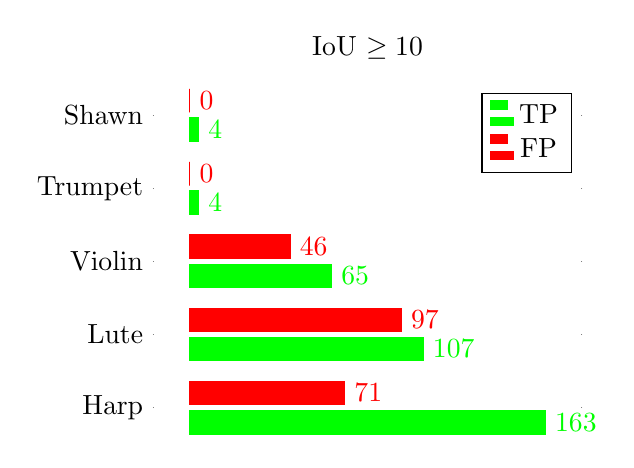
\begin{tikzpicture}
  \begin{axis}[title  = IoU $\geq 10$,
    xbar,
    bar width=.3cm,
    y axis line style = { opacity = 0 },
    axis x line       = none,
    tickwidth         = 0.5pt,
    width=7cm,
    symbolic y coords = {Harp, Lute, Violin, Trumpet, Shawn},
    ytick= data,
    nodes near coords,
  ]
  \addplot [color=green,fill ] coordinates {(163,Harp) (107,Lute) (65,Violin) (4,Trumpet) (4,Shawn)};
  \addplot [color=red,fill] coordinates {(71,Harp) (97,Lute) (46,Violin) (0,Trumpet) (0,Shawn)};
\legend{TP,FP}
\end{axis}
\end{tikzpicture}
 \end{minipage}
 \hspace{3cm}
\begin{minipage}{.5\textwidth}
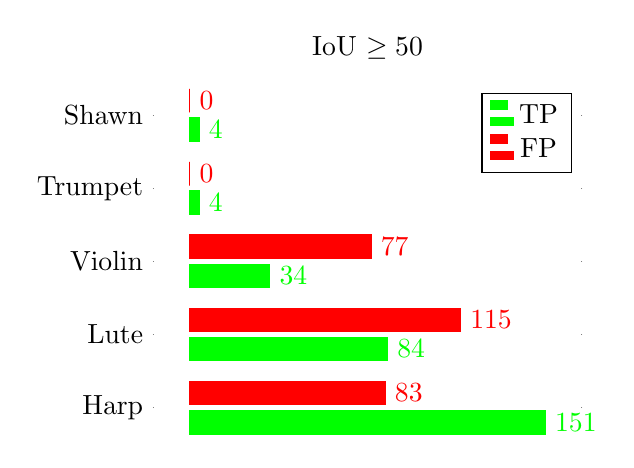
\begin{tikzpicture}
  \begin{axis}[title  = IoU $\geq 50$,
    xbar,
    bar width=.3cm,
    y axis line style = { opacity = 0 },
    axis x line       = none,
    tickwidth         = 0.5pt,
    width=7cm,
    symbolic y coords = {Harp, Lute, Violin, Trumpet, Shawn},
    ytick=data,
    nodes near coords,
  ]
  \addplot [color=green,fill] coordinates {(151,Harp) (84,Lute) (34,Violin) (4,Trumpet) (4,Shawn)};
  \addplot [color=red,fill] coordinates {(83,Harp) (115,Lute) (77,Violin) (0,Trumpet) (0,Shawn)};
\legend{TP,FP}

\end{axis}
\end{tikzpicture}
 \end{minipage}
 

